\section{Experiments}
\label{sec:experiments}

We organize the experiments around three questions: whether the regime-local specialists support autonomous prediction, whether
physical-space fusion improves prediction near regime transitions, and how the main local architectural choices affect prediction.
The three incompressible-flow benchmarks play complementary roles in answering these questions. All are two-dimensional systems in which varying the Reynolds number traverses steady, Hopf-onset, and periodic regimes. The circular-cylinder benchmark provides matched local controls and an initialization audit, the centered-square benchmark evaluates cross-regime routing and fusion in the $S$--$H$ and $H$--$P$ overlaps, and the fluidic-pinball benchmark provides the autonomous comparison with a classical POD--Galerkin ROM. Table~\ref{tab:benchmark_summary} summarizes the benchmark scope and roles. The reported chart-wise splits use complete parameter trajectories rather than individual snapshots or rollout windows; chart-wise parameter ranges and split counts are reported in Appendix~\ref{app:implementation}.

We report relative physical-field errors $E_u$ and $E_p$ in percent; their weighted definitions and benchmark-specific aggregation rules are given in Appendix~\ref{app:implementation}. For routing and fusion comparisons, $E_{\mathrm{joint}}=E_u+E_p$. The sum of displayed component errors can differ slightly from the reported joint error because values are rounded independently. The new Circular controls and Square cache-based reevaluation use
POD-reconstructed reference fields, excluding the original CFD projection
remainder. We distinguish training failure, validation rejection, and
non-finite test rollout; an unavailable result is not automatically a
divergence. 

\par
\begin{table}[H]
\centering
\caption{
Experimental scope and benchmark roles.
Local rank pairs $(r_u,r_p)$ are ordered $S,H,P$.
Horizons are ordered $S,H,P$ except for the new Circular H/P controls.
Additional overlap and periodic-core settings are specified in their
respective comparisons.
}
\label{tab:benchmark_summary}
\small
\setlength{\tabcolsep}{4pt}
\begin{tabular}{@{}>{\raggedright\arraybackslash}p{2.15cm}
>{\raggedright\arraybackslash}p{1.30cm}
>{\raggedright\arraybackslash}p{4.05cm}
>{\raggedright\arraybackslash}p{1.80cm}
>{\raggedright\arraybackslash}p{2.50cm}@{}}
\toprule
Benchmark & $Re$ range & Local ranks ($S,H,P$) & Rollout horizons & Primary role \\
\midrule
Circular cylinder
& 20--200
& $(32,32),\ (32,32),\ (32,32)$
& H/P: $24,48$
& Matched local controls \\
\addlinespace
Centered square
& 50--150
& $(5,4),\ (11,11),\ (28,26)$
& $16/48/24$
& Cross-regime routing/fusion \\
\addlinespace
Fluidic pinball
& 10--60
& $(4,3),\ (5,5),\ (17,16)$
& $56/56/32$
& Autonomous ROM baseline \\
\bottomrule
\end{tabular}
\end{table}
\par



\subsection{Do local specialists support accurate autonomous rollouts?}

We first examine whether the regime-local specialists maintain accurate predictions under autonomous rollout on the fluidic-pinball benchmark. Table~\ref{tab:pinball_autonomous} compares the learned specialists with a classical POD--Galerkin ROM over the Steady, Hopf, and Periodic regimes.

RAL-MoE-ROM achieves low physical-field errors across all four evaluation settings. In the Hopf and Periodic settings where POD--Galerkin errors are reported, the learned specialists consistently reduce both velocity and pressure
errors, with the largest differences appearing in pressure. For example, the Hopf joint error decreases from $48.94\%$ to $2.085\%$, while the standard Periodic error decreases from $43.20\%$ to $0.8415\%$. The longer-horizon Periodic-core evaluation shows the same trend, with $E_{\mathrm{joint}}$ reduced from $41.91\%$ to $1.672\%$. Together, these results show that the learned specialists maintain low physical-field error over the evaluated autonomous horizons.

\par
\begin{table}[H]
\centering
\caption{
Autonomous local-specialist prediction on the fluidic-pinball benchmark. Errors are physical-field percentages; lower is better. Periodic-core denotes the longer-horizon periodic evaluation; complete protocol details are given in Appendix~\ref{app:pinball}. A dash indicates that no baseline error is reported.
}
\label{tab:pinball_autonomous}
\small
\setlength{\tabcolsep}{5pt}
\begin{tabular}{@{}llrrr@{}}
\toprule
Evaluation setting & Model & $E_u$ & $E_p$ & $E_{\mathrm{joint}}$ \\
\midrule
Steady ($K=56$)
& POD--Galerkin
& -- & -- & -- \\
& RAL-MoE-ROM
& 0.2247 & 0.7593 & 0.9840 \\
\addlinespace

Hopf ($K=56$)
& POD--Galerkin
& 0.4378 & 48.50 & 48.94 \\
& RAL-MoE-ROM
& 0.0995 & 1.986 & 2.085 \\
\addlinespace

Periodic ($K=32$)
& POD--Galerkin
& 1.641 & 41.56 & 43.20 \\
& RAL-MoE-ROM
& 0.2897 & 0.5518 & 0.8415 \\
\addlinespace

Periodic-core ($K=56$)
& POD--Galerkin
& 2.555 & 39.36 & 41.91 \\
& RAL-MoE-ROM
& 0.6222 & 1.050 & 1.672 \\
\bottomrule
\end{tabular}
\end{table}
\par

A complementary POD--DeepONet experiment further separates one-step prediction from autonomous rollout.
The model attains $E_u=1.5921\%$ and $E_p=23.3447\%$ on 4,228 held-out one-step pairs, but only one of 28 held-out trajectories completes the prescribed autonomous rollout evaluation. Because its temporal cadence differs from that of the Periodic specialist, we use this result only to contrast one-step prediction with autonomous rollout, rather than as a matched long-horizon accuracy comparison (Appendix~\ref{app:pinball}).





\subsection{Does physical-space fusion improve prediction in regime overlaps?}
To evaluate the second routing level while holding the local specialists fixed, we compare the centered-square $S$--$H$ and $H$--$P$ overlaps at $K=24$ (Table~\ref{tab:routing_fusion}). We compare hard E2 Top-1 routing with two simple fusion rules, the Equal blend and the E2-probability blend, together with the learned T2-C gate; a diagnostic convex oracle provides an a posteriori reference. To test whether T2-C benefits specifically from physical-history information, we additionally include an architecture-matched T2-C $\mu$-only ablation. The same gate architecture and optimization protocol are retained, but the standardized history-descriptor channels are set to zero. This preserves the gate parameterization and trainable parameter count while removing history information.


The $\mu$-only ablation reveals that parameter conditioning alone has overlap-dependent value. For $S$--$H$, its joint error is essentially unchanged relative to the E2-probability blend ($2.1846\%$ versus $2.1847\%$), whereas for $H$--$P$ it improves the same baseline from $1.6618\%$ to $1.1504\%$. Adding the physical-history descriptor improves both overlaps further, reducing $E_{\mathrm{joint}}$ to $1.1958\%$ and $0.8465\%$, respectively. Relative to the a posteriori best fixed-specialist reference, full T2-C reduces joint error by $30.9\%$ on $S$--$H$ and $29.9\%$ on $H$--$P$. Relative to the deployable E2 Top-1 router, the corresponding reductions are $30.9\%$ and $54.2\%$. The terminal scores are numerically close to the diagnostic convex reference, whose full-window objective differs from this terminal metric; this is not evidence of terminal optimality. Figure~\ref{fig:square_overlap} summarizes the paired gate-seed results; reconstructed fields showing both candidates are given in Appendix~\ref{app:square}.

Across three paired gate-training seeds, full T2-C outperforms the architecture-matched $\mu$-only gate in every run for both overlaps.
Across the three paired runs, the mean reduction relative to $\mu$-only is $45.3\%$ for $S$--$H$ and $26.2\%$ for $H$--$P$. Full T2-C yields
$E_{\mathrm{joint}}=1.1957\pm0.0001\%$ on $S$--$H$ and $0.8500\pm0.0035\%$ on $H$--$P$, where $\pm$ denotes the sample standard
deviation across the three gate-training seeds. Only gate training is repeated across seeds; the specialists, E2 router, candidate rollouts, data splits, normalization, and optimization protocol are fixed. These statistics therefore characterize gate-training variability rather than full-pipeline uncertainty. Component-wise errors and seed-level results are reported in Appendix~\ref{app:square}, with the corresponding fluidic-pinball overlap study in Appendix~\ref{app:pinball}.


\par
\begin{table}[H]
\centering
\caption{
Validation-selected cross-regime routing and fusion on the centered-square benchmark at $K=24$. Entries are terminal-step $E_{\mathrm{joint}}$ (\%); lower is better. T2-C $\mu$-only uses the same gate architecture with all standardized history-descriptor channels set to zero. The oracle is an a posteriori convex reference and is not available at inference. Three-seed gate-training variability is reported separately in
Appendix~\ref{app:square}. Bold marks the best deployable method in this validation-selected comparison.
}
\label{tab:routing_fusion}
\small
\setlength{\tabcolsep}{3.5pt}
\begin{threeparttable}
\begin{tabular}{@{}lrrrrrrr@{}}
\toprule
Overlap & Best fixed$^\ast$ & E2 Top-1 & \shortstack{Equal\\blend} & \shortstack{E2-probability\\blend} & \shortstack{T2-C\\$\mu$-only} & T2-C & \shortstack{Convex\\oracle}\\
\midrule
$S$--$H$ & 1.7298 & 1.7298 & 3.0321 & 2.1847 & 2.1846 & \textbf{1.1958} & 1.1842 \\
$H$--$P$ & 1.2079 & 1.8473 & 1.6146 & 1.6618 & 1.1504 & \textbf{0.8465} & 0.8384 \\
\bottomrule
\end{tabular}
\begin{tablenotes}[flushleft]
\footnotesize
\item[$\ast$] Best fixed denotes the a posteriori fixed-specialist reference selected by aggregate evaluation error over the corresponding overlap (Hopf for $S$--$H$, Periodic for $H$--$P$). It is not a routing strategy available at inference.
\end{tablenotes}
\end{threeparttable}
\end{table}
\par


\begin{figure}[H]
\centering
% Source: audited three-gate-seed full-window means; no field pixels generated.
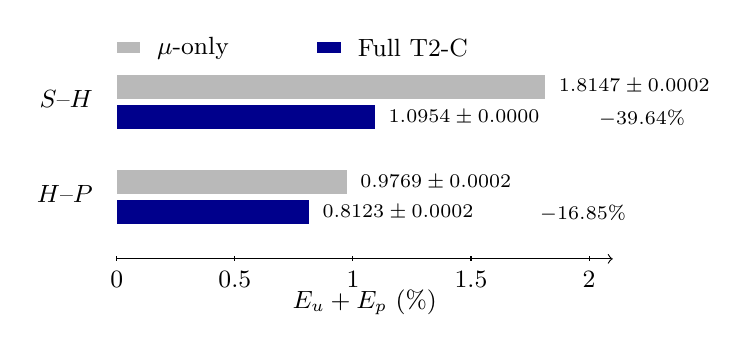
\begin{tikzpicture}[x=3cm,y=0.55cm,font=\small]
\draw[->] (0,0)--(2.1,0);
\node at (1.05,-1.0) {$E_u+E_p$ (\%)};
\foreach \t in {0,0.5,1,1.5,2} {
 \draw (\t,0.06)--(\t,-0.06) node[below] {\t};
}
\node[anchor=east] at (-0.06,3.7) {$S$--$H$};
\node[anchor=east] at (-0.06,1.5) {$H$--$P$};
\fill[gray!55] (0,3.7) rectangle (1.814699,4.25);
\fill[blue!55!black] (0,3.0) rectangle (1.095351,3.55);
\fill[gray!55] (0,1.5) rectangle (0.976939,2.05);
\fill[blue!55!black] (0,0.8) rectangle (0.812343,1.35);
% Display precision only; bar geometry retains the original means.
% The displayed 0.0000 is rounded from a nonzero standard deviation.
\node[anchor=west,font=\scriptsize] at (1.83,3.975) {$1.8147\pm0.0002$};
\node[anchor=west,font=\scriptsize] at (1.11,3.275) {$1.0954\pm0.0000$};
\node[anchor=west,font=\scriptsize] at (0.99,1.775) {$0.9769\pm0.0002$};
\node[anchor=west,font=\scriptsize] at (0.83,1.075) {$0.8123\pm0.0002$};
\fill[gray!55] (0,4.75) rectangle (0.1,5.0);
\node[anchor=west] at (0.13,4.87) {$\mu$-only};
\fill[blue!55!black] (0.85,4.75) rectangle (0.95,5.0);
\node[anchor=west] at (0.98,4.87) {Full T2-C};
\node[anchor=west,font=\scriptsize] at (2.0,3.25) {$-39.64\%$};
\node[anchor=west,font=\scriptsize] at (1.75,1.05) {$-16.85\%$};
\end{tikzpicture}

\caption{Full-window joint errors at $K=24$ for both centered-square
overlaps. Values are mean $\pm$ sample standard deviation across three
paired gate-training seeds with all candidate trajectories fixed.
The reductions are relative to the architecture-matched $\mu$-only gate.
The field comparisons in Appendix~\ref{app:square} include both
specialists, including the stronger Periodic candidate in $H$--$P$.}
\label{fig:square_overlap}
\end{figure}

The full-window comparison in Figure~\ref{fig:square_overlap} gives the
same direction of effect as the terminal metric: history conditioning
reduces the three-seed mean joint error by $39.64\%$ in $S$--$H$ and
$16.85\%$ in $H$--$P$. These results condition on fixed candidates.
The frozen-checkpoint reevaluation also improves on training-fitted
constant mixing weights and constant-logit offsets
(Appendix~\ref{app:square}).

\subsection{What do matched local controls establish?}

We reevaluate Circular H/P models with common held-out windows and
POD-reconstructed reference fields. The Dense control matches the active
parameter budget of the proposed model; the structured control removes
input-dependent routing. This is distinct from the earlier
Vanilla-FNN-MoE, DataOnly-MoE, and Global MoE comparison, whose summary and
min--max tables are replaced here because their historical aggregation
could not be fully reconciled. The new results do not retroactively
validate those old statistics or isolate every architectural factor.

\begin{table}[H]
\centering
\caption{Circular Periodic controls: full-window mean physical-field
errors (\%) at $K=24$, against POD-reconstructed truth. Entries are mean
$\pm$ sample standard deviation over seeds 1248, 1600, and 2026; all
listed neural configurations have 3/3 accepted seeds. Repaired denotes
the changed quadratic-branch initialization.}
\label{tab:circular_full_reorg}
\small
\setlength{\tabcolsep}{4pt}
\begin{tabular}{@{}lccc@{}}
\toprule
Model & $E_u$ & $E_p$ & $E_u+E_p$\\
\midrule
Proposed, original & $0.5731\pm0.3638$ & $2.3060\pm1.3681$ & $2.8791\pm1.7269$\\
Proposed, repaired & $0.5814\pm0.3949$ & $2.4854\pm1.4427$ & $3.0667\pm1.8373$\\
Dense, active-matched & $\mathbf{0.2446\pm0.0323}$ & $\mathbf{1.0805\pm0.1946}$ & $\mathbf{1.3251\pm0.2268}$\\
Structured, original & $0.5178\pm0.2667$ & $2.3489\pm1.1688$ & $2.8666\pm1.4342$\\
Structured, repaired & $0.5429\pm0.2783$ & $2.3168\pm1.0315$ & $2.8598\pm1.3081$\\
\bottomrule
\end{tabular}
\end{table}

The Dense control is more accurate than both proposed configurations at
$K=24$ and $K=48$ (Appendix~\ref{app:circular}). The routing-free
structured control is close to the proposed model. Thus this study does
not identify sparse local routing as a source of Periodic accuracy under
the matched active-parameter budget.

A checkpoint audit found that the original Circular quadratic branches
remained zero because both multiplicative factors were initialized at
zero. Keeping one factor random activates the branch but does not improve
Periodic accuracy consistently. For Hopf, two of six repaired FP32 runs
still develop non-finite gradients, leaving two accepted seeds per
architecture. We report their errors as accepted-only descriptive
statistics, not complete three-seed estimates.

A regularized polynomial OpInf adaptation is competitive on Hopf
($K=24$ joint error $0.03870\%$) but performs poorly on Periodic
($114.0941\%$). Its pressure map, derivative estimation, and validation
search are documented in Appendix~\ref{app:circular}; these results do
not establish a general advantage over the OpInf method family.

\paragraph{Computational scope.}
Per-decision active parameter counts characterize conditional execution,
not latency. A batch-one native Circular Periodic $K=48$ rollout with
physical decoding takes a median $2.1848$ s for proposed, compared with
$0.6579$ s for Dense. This diagnostic excludes initialization, outer
routing, descriptor construction, and fusion. It therefore provides
neither an end-to-end runtime nor a FOM speedup
(Appendix~\ref{app:parameter_counts}).
